\documentclass{cumcm}
\begin{document}
\begin{minipage}{0.9\textwidth}
\centering\LARGE\textbf{“同心协力”策略研究}

\end{minipage}
\begin{abstract}
本题在于考察分析同心球项目中不同情境下,通过调整团队队员发力的时机及力度,找出团队协作的最佳策略,使排球在鼓面上能持续颠起。\par
\begin{itemize}
\item \textbf{问题一分析}\quad\\
\item \textbf{问题二分析}\quad\\
\item \textbf{问题三分析}\quad\\
\item \textbf{问题四分析}\quad\\
\end{itemize}
\textbf{关键词} \quad MATLAB \quad 同心球 \quad 
\end{abstract}

\newpage
\section{问题重述}
\subsection{问题背景}
“同心协力”是一项需要团队高度协作的项目,不仅考察队员之间的默契程度,还锻炼了队员在压力环境中的心理承受能力,近年来受到了人们的热烈追捧。该项目的道具是一面在鼓身沿圆周均匀固定了多根绳子的牛皮双面鼓,以及一个富有弹性、气密性好的专用排球。项目开始时,团队成员每人牵拉一根绳子的末端,使鼓面保持水平,然后将球从鼓面正中心放下,队员找准时机同时用力将球颠起,使其能在鼓面上持续跳动而不落地,最终颠球次数最多的队伍获胜。
\subsection{问题的提出(题目重述)}
项目的目标是使球连续颠起次数尽可能多。现给定相关参数,包括所用双面鼓及排球的质量,鼓面直径,鼓身高度。同时要求团队队员人数不少于$8$人,各队员之间最小距离不小于$60cm$。排球最开始从鼓面中心正上方$40cm$处竖直下落,之后被颠起高度离鼓面距离应不小于$40cm$,否则项目终止。试通过数学建模,给出最佳策略。
\begin{enumerate}[(1)]
\item 假设每个队员都可以精确控制用力方向、时机和力度,讨论在此理想状态下团队的最佳协作策略,并给出该策略下的颠球高度。
\item 现实情况下,由于各队员之间用力不同,鼓面会出现一定程度的倾斜。试通过给定的参考数据,建立模型考察队员的发力时机和力度与某一特定时刻的鼓面倾斜角度关系。
\item 根据问题$2$中考虑了现实情况的模型,对问题$1$的策略做出适当调整。
\item 实际中,当鼓面发生倾斜时,球的跳动方向也不再竖直。现给定相关数据,计算出在可精确控制条件下所有队员的发力时机及力度,使球调整为竖直状态弹跳,并分析在现实情况中这种调整策略的实施效果。
\end{enumerate}

\section{模型假设}
\begin{enumerate}
\item 假设每根绳子均为柔性绳,每根绳子长度相同。
\item 不考虑风力以及空气阻力对排球运动的影响。
\item 当地重力加速度为$9.8kg/m^2$。
\item 排球是一个直径为$204mm$的五号标准排球。
\item 将排球视为一个均匀球壳。
\item 每位队员所隔距离相同,且手离地面高度相同,即各力作用位置沿鼓均匀分布。
\end{enumerate}

\section{符号说明}
表\ref{table-symbol}列出了本文需要的符号。
\begin{table}[H]
  \centering
  \caption{符号说明}\label{table-symbol}
  \begin{tabular*}{\textwidth}{c|c|c|c}
  \hline
  符号 & 符号描述 & 符号 & 符号描述\\
  \hline
  $l$ & 绳子长度 &  $\varphi_0$ & 鼓在平衡位置时绳子与竖直方向夹角\\
  $h$ & 鼓距离地面高度 & $\varphi$ & 运动过程中绳子与竖直方向夹角\\
  $v_{00}$ & 碰撞前鼓的速度 &  $x_{10}$ & 球从最高处落下到碰撞时的位移\\
  $v_{01}$ & 碰撞后鼓的速度 &  $x_{00}$ & 鼓从平衡位置到碰撞时的位移\\
  $v_{10}$ & 碰撞前球的速度 & $x_{01}$ & 鼓自由落体的位移\\
  $v_{11}$ & 碰撞后球的速度 & $x_{02}$ & 鼓减速回到平衡位置的位移\\
  $F_i$ & 第$i$位队员施加力的大小 & $v_{02}$ & 鼓自由落体结束时的速度\\
     \\
  \hline
  \end{tabular*}
\end{table}


\section{问题分析}
\subsection{问题1分析}
题一是一个运动过程分析问题。我们假设在初始条件下鼓处于平衡位置,记为$s_0$。我们将一次颠球过程分为三个阶段:在第一阶段每位队员施加竖直向上的力使鼓向上运动,到达$s_1$与排球碰撞,此时鼓上升高度为$x_{00}$,球下降的高度为$x_{10}$。在碰撞前鼓有一个竖直向上的速度$v_{00}$,球有一个竖直向下的速度$v_{10}$。我们考虑两者碰撞过程在瞬间完成,碰撞后鼓速度变为$v_{01}$,球速度变为$v_{11}$,方向均为竖直向上。在第二阶段,排球继续上升,而鼓做自由落体运动,运动方向为先上升后下降,到达$s_2$,此时鼓速度为$v_{02}$,与碰撞处的高度差为$x_{01}$,运动时间为$t_{01}$。在第三阶段,队员施加力使鼓做减速运动,最终回到平衡位置,同时排球到达最高处,结束时鼓与排球的速度都为$0$。运动分析图如下所示(为方便查看将鼓运动位移放大):
\begin{figure}[H]
\centering
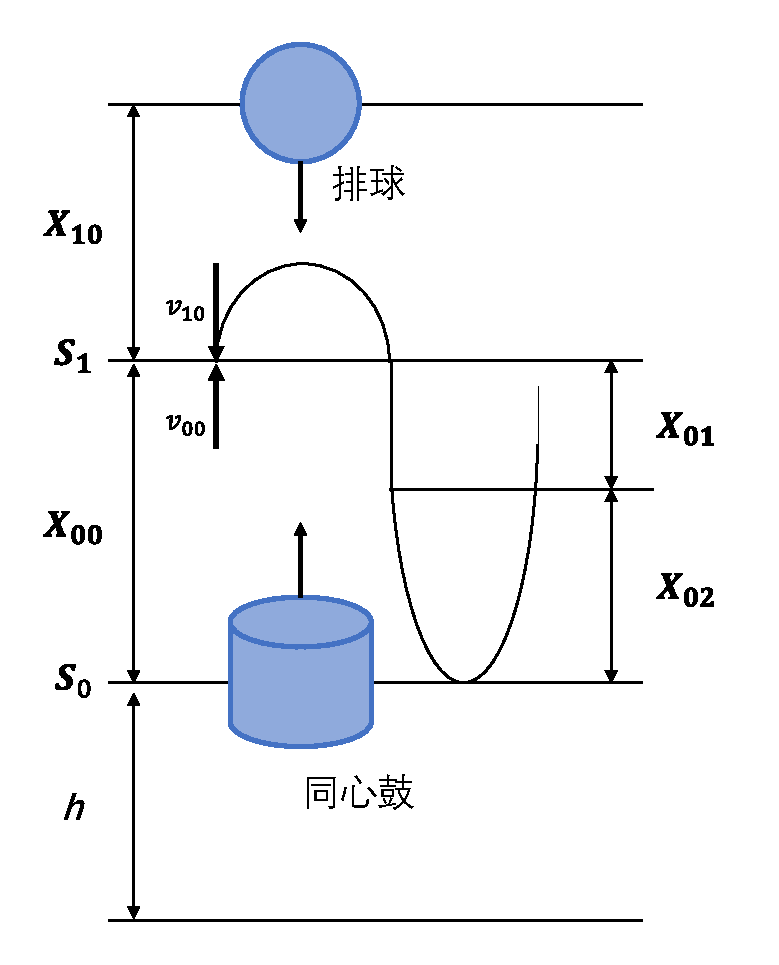
\includegraphics[width=0.5\textwidth]{img/question1.png}
\caption{问题一运动过程示意图}\label{fig-buoy}
\end{figure}

\subsection{问题2分析}
\subsection{问题3分析}
\subsection{问题4分析}


\subsection{问题1的解答}
\begin{enumerate}
\item \textbf{绳长计算}\\
我们假设团队队员共有$n$人,每人之间的距离为$60cm$,忽略绳子在鼓身上的固定端之间的距离,将鼓看成一个质点。则固定端与两队员队员所站位置可构成水平的等腰三角形,三角形顶角为$\frac{360^{\circ}}{n}$,三角形底角角度为($90^{\circ}\frac{180^{\circ}}{n}$),如下图所示:
\begin{figure}[H]
\centering
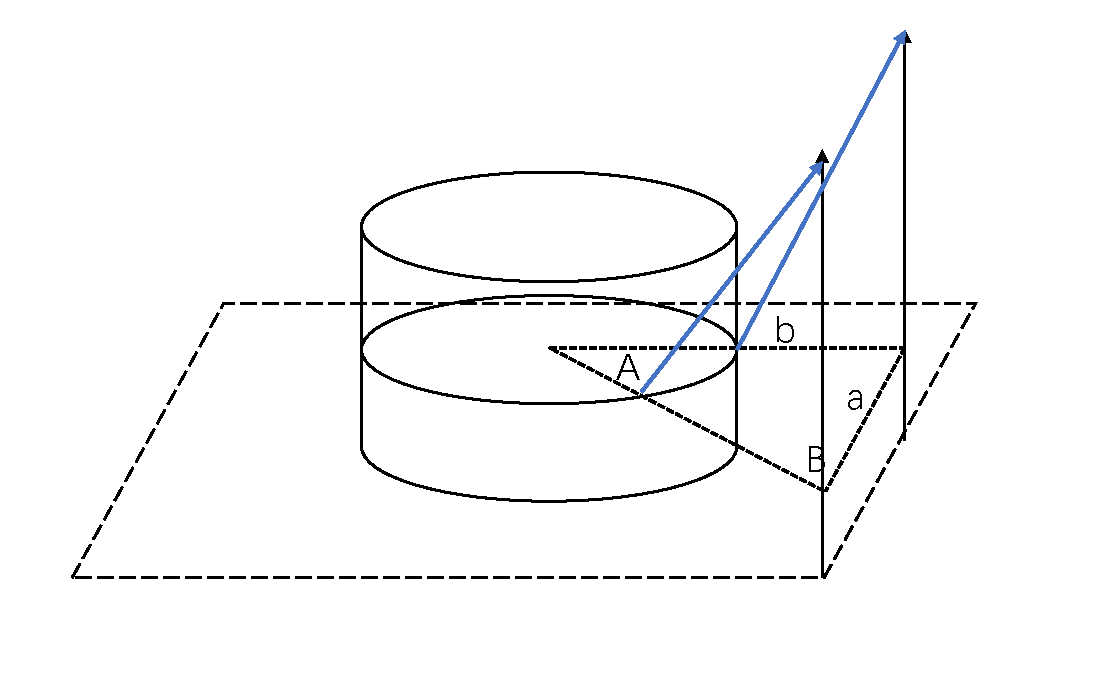
\includegraphics[width=0.5\textwidth]{img/string.png}
\caption{绳长计算示意图}
\end{figure}
由正弦定理可得:
\begin{displaymath}
\frac{a}{sinA}=\frac{b}{sinB}
\end{displaymath}
即:
\begin{displaymath}
\frac{60}{sin({\frac{360^{\circ}}{n}})}=\frac{b}{sin({90^{\circ}-\frac{180^{\circ}}{n}})}
\end{displaymath}
解得$b$的长度为:
\begin{displaymath}
b=\frac{30}{sin( \frac{180^{\circ}}{n})}
\end{displaymath}
又因为绳子与竖直方向夹角为$\varphi$,所以绳子长度可以表示为:
\begin{displaymath}
l=\frac{b}{sin\varphi}=\frac{30}{sin(\frac{180^{\circ}}{n})sin\varphi}
\end{displaymath}
\item
\end{enumerate}
$$\text{m0} \text{v00}-\text{m1} \text{v11}=\text{m0} \text{v01}+\text{m1} \text{v11},\text{Null}\frac{\text{v11}-\text{v01}}{\text{v00}+\text{v11}}=e,\text{Null}a \text{v11}=g \text{v00},\text{Null}\frac{\text{v11}}{g}=\frac{\text{v02}}{\text{a2}}+\frac{\text{v01}+\text{v02}}{g},\text{Null}\frac{\text{v00}^2}{2 \text{a1}}+\frac{\text{v11}^2}{2 g}=0.4,\text{Null}\frac{\text{v02}^2}{2 \text{a2}}+\frac{\text{v02}^2-\text{v01}^2}{2 g}+\frac{\text{v11}^2}{2 g}=0.4
$$
\subsection{问题2的解答}
\subsection{问题3解答}
\subsection{问题4解答}
\section{模型总结}

\subsection{模型优点}

\subsection{模型缺点}


\bibliographystyle{plain}
\bibliography{ref}
\begin{thebibliography}{99}
\bibitem{1}
\bibitem{2}
\end{thebibliography}

\newpage
\appendix
\textbf{附录}
\section{模型求解代码}

\end{document}
